% !TEX root = ../main.tex

\chapter{Presentation of the company} % (fold)
\label{chp:presentation}

\section{The company} % (fold)
\label{sec:company}

Algolia~\cite{algolia-home} is a hosted Search as a Service (SaaS) provider. The company aims to improves user and developer experience on a global scale: increasing the accuracy and speed of searching for the users and empowering developers by providing an extended service with comprehensive documentation and support. The speed and low latency of queries is provided by 47 bare-metal data centers across 15 regions and relevant search results are enabled by a custom search engine, built from scratch.

Algolia has over 3000 paying customers from several industries, like Birchbox, LVMH and The Kooples in the e-commerce space, Twitch, Periscope, Vevo and Medium in the media space, Stripe, Product Hunt and Mailjet in the developer tools branche, as well as a lot more clients in harder to define areas. Algolia also offers a permanently free plan which is used over 6000 applications, ranging from small websites to bigger community projects, like the documentation on frameworks like React.

Algolia is a global oriented culture-first company. These core values are translated in practical work organization and work-ethics where ownership of each team member plays a central role.

\subsection{History}
\label{sub:history}

Algolia is a privately held startup founded in 2012 in Paris by Nicolas Dessaigne and Julien Lemoine, who both have years of experience maintaining adn writing search engines. Thinking globally the founders didn't limit their search area for clients and investors to Europe.

After two very successful investment rounds in the US and the growing number of clients in the US --- two-thirds of revenues come from United states \cite{less-mis} --- the headquarters moved to San Francisco, US in 2014, although all of the development still happens in Paris. 

Both offices work in strong co-creation as there is direct collaboration between the clients, their developers and the Algolia developers. As the time difference between the San Francisco headquarters and the Paris office is nine hours, communication was sometimes challenge. In spring 2017 two satellite offices opened in New York and Atlanta on the Eastern Coast of the US. These offices bridge the time difference and improve internal and external communication.

At the time of writing Algolia has 113 employees: 34 in the San Francisco headquarters, 70 in the Paris office and 9 in the satellite offices in New York and Atlanta. The company is expanding rapidly and looking for effective ways to keep this exponential growth in balance with the company’s culture and values described in the next item.

\subsection{Company culture}
\label{sub:company_culture}

Both founders Nicolas Dessaigne and Julien Lemoine had similar work experiences as developers in large multinational companies. In these companies they experienced different cultures. This made them convinced in what they didn't want for their own company and made them look for inspiration and an alternative.

In the beginning of the Twenty-First Century academics and entrepreneurs were looking for an alternative to the top down culture in companies and organizations. This top down organizational model originated from the exponential growth of businesses during the industrial revolution and the need to motivate and monitor the workers to ensure a high production rate as well as the quality of products.

%% lijkt twintigste-eeuw

As many start ups Algolia’s founders were inspired by these authors and companies experimenting with and innovating work organization. For Algolia ``Freedom, inc.''\cite{freedom-inc} was and still is the reference work to build and maintain the culture of the company. Ownership became the cornerstone for Algolia. Every team member is free to take initiative and to make decisions. Nicolas Dessaigne describes it as follows in the article ``How Algolia built a Culture-First Company around Ownership'':

\begin{quote}
We want owners, we want people who act as if it was their company, people who realize that, actually, it is their company~\cite{culture-first}~.
\end{quote}

\subsection{Values}
\label{sub:values}

As a culture first company it was important to capture and anchor the values of Algolia from the beginning. In the period imagining Algolia the founders not only thought about their product but also on how they envisioned working together with each other and with their future employees. In doing so they secured their culture against the influences of future growth. Company decisions and the way employees work are designed around these values.

\begin{figure}[H]
  \centering
  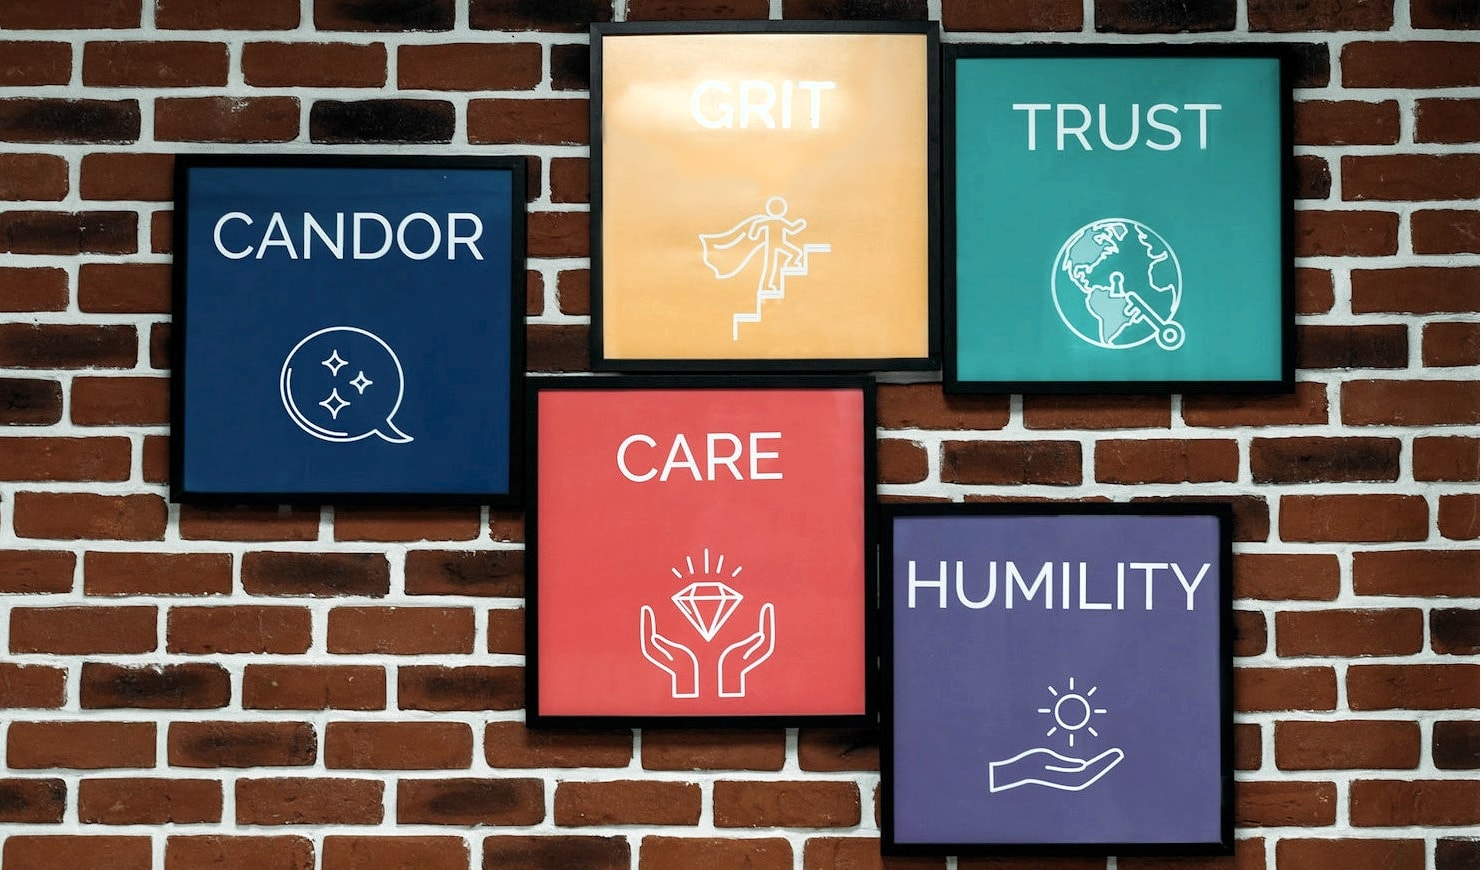
\includegraphics[width=0.5\textwidth]{values.jpg}
  \caption{The core values, as hung out in the Algolia office\cite{culture-first}}
  \label{figure:values}
\end{figure}

Following core values make the backbone of Algolia's company culture: Grit, Trust, Care, Candor and Humility~\cite{algolia-values}~. 

\subsubsection{Grit}
\label{ssub:grit}

%% find citation for grit
\begin{definition}
Grit is the tendency to sustain interest in and effort toward very long-term goals\cite{Duckworth201605}
\end{definition}

\begin{wrapfigure}{l}{0.25\textwidth}
  \centering
  
\includegraphics[scale=0.25]{grit.pdf}
\end{wrapfigure}

\paragraph{Translated in the Algolia culture book}

\textbf{Grit} in everything we do. We have the determination to go further. We think long-term and constantly strive to be better, even if things don’t always go as expected. We know there's always room for improvement and are constantly pushing ourselves further~\cite{algolia-careers}~.

\paragraph{What it means for employees} 

Goals for employees are set high. Once an employee or intern is accepted by the company, they gets full responsibility and are seen and accepted as a team member. This makes working at Algolia challenging and exciting.

\subsubsection{Trust}
\label{ssub:trust}

\begin{definition}
verb; to believe that someone is good and honest and will not harm you, or that something is safe and reliable\cite{cambridge-trust}
\end{definition}

\begin{wrapfigure}{l}{0.25\textwidth}
  \centering
  
\includegraphics[scale=0.25]{trust.pdf}
\end{wrapfigure}

\paragraph{Translated in the Algolia culture book}

Have \textbf{Trust} in yourself and others. Trust is one of the cornerstones of Algolia. We have trust in our people, and we build trust with our customers. We listen, follow through and keep our words. We are fully transparent within the company and with our customers~\cite{algolia-careers}~.

\paragraph{What it means for employees}

This goal is very important to facilitate the ownership culture that Algolia wants. For example intermediate and hierarchic levels are limited to the bare minimum. Another example is how the company copes with problems. Instead of treating the problem by creating barriers so that the problem doesn't reproduce itself, it is treated as an exceptional situation. The transparency of the company is another example of the innovative character of Algolia: internal publishing of everyone's salary (founders included), making all tools publicly available, all developed code is shared with the whole team, \dots

\subsubsection{Care}
\label{ssub:care}

\begin{definition}
noun (protection); the process of protecting someone or something and providing what that person or thing needs\cite{cambridge-care}
\end{definition}

\begin{wrapfigure}{l}{0.25\textwidth}
  \centering
  
\includegraphics[scale=0.25]{care.pdf}
\end{wrapfigure}

\paragraph{Translated in the Algolia culture book}

\textbf{Care} Passionately. We want the best for our customers and our people. We go above and beyond to make our customers and people happy. We have each other's backs and help one another succeed~\cite{algolia-careers}~.

\paragraph{What it means for employees} 

Algolia takes good care of their clients and offers several levels of support depending on the chosen customer plan. There is direct communication between the client, his developer and the Algolia developer. This makes the expectations of the client transparent for the Algolia developer.

An employee is never the sole responsible for a project, but is a member of a team or squad. This multifunctional team supports all aspects of a project: from the design to elaborating reflecting and modifying.

Strengthening the social cohesion between team members in the office is done by organizing weekly after work drinks in the office, regular meet-ups are held, newcomers get a warm welcome, \dots

\subsubsection{Candor}
\label{ssub:candor}

\begin{definition}
noun; the quality of being open and honest in expression; frankness~\cite{oxford-candor}~.
\end{definition}

\begin{wrapfigure}{l}{0.25\textwidth}
  \centering
  
\includegraphics[scale=0.25]{candor.pdf}
\end{wrapfigure}

\paragraph{Translated in the Algolia culture book}

Be radical in your \textbf{Candor}. We are open and honest. We give each other praise and criticism because we personally care and want to challenge each other and help one another grow~\cite{algolia-careers}~.

\paragraph{What it means for employees} 

In Algolia there is an open culture and communication is direct and respectful between all team members. This is also reflected in one-on-one meetings, where a preference for telling things like they are, instead of avoiding issues is shown.

\subsubsection{Humility}
\label{ssub:humility}

\begin{definition}
noun; the quality of having a modest or low view of one's importance~\cite{oxford-humility}~.
\end{definition}

\begin{wrapfigure}{l}{0.25\textwidth}
  \centering
  
\includegraphics[scale=0.25]{humility.pdf}
\end{wrapfigure}

\paragraph{Translated in the Algolia culture book}

Behave with \textbf{Humility}. We want to see our teammates succeed as much as we do ourselves. We do not think we are better than other people and do not focus only on ourselves~\cite{algolia-careers}~.

\paragraph{What it means for employees} 

Ego is not seen as a positive thing at Algolia. Achievements done by a specific employee are always attributed to the team.

\subsubsection{Teamwork}

Algolia strongly believes in working as a team. This teamwork is facilitated in the way decisions are made in total transparency, how offices work and the work is organised. Where many companies choose to promote teleworking Algolia chooses for working together in an open office so that formal and informal consultation between co-working is facilitated.

The four offices work as one global team, not four independent teams. To overcome a future language barrier English has always been the working language in the Paris and US offices, even if none of the founders and co-workers in the beginning were native speakers. Also employees are encouraged to travel to one of the other offices once a year. 

\subsection{Mission statement and vision}
\subsubsection{Mission statement of Algolia}

The first mission statement of Algolia was:

%%src

\begin{quote}
Make the path to finding and exploring content and efficient, enjoyable and rewarding experience on all websites and apps.
\end{quote}

After a cooperative process where all the employees could contribute an actualized mission statement was designed in the summer of 2016. The following mission statement is:

\begin{quote}
Relevant content at the speed of thought
\end{quote}

\subsubsection{Vision of Algolia}

Algolia helps their users to deliver an intuitive search-as-you-type experience on their websites and mobile apps. Basically, Algolia makes finding things easier. Algolia is a customer-focused, dev-centric company dedicated to changing the way people think about search.

\subsection{Operational goals}

\subsubsection{Enable to find data at the speed of thought}

Algolia gives the users of their clients' websites or mobile applications fast access to what they’re looking for. The aim of Algolia is to serve the best results at the speed of a keystroke.

\begin{itemize}
  \item Making searching content on a website or mobile application find-as-you-type fast, which requires extreme speed and optimized relevance.
  \item Getting results in milliseconds, refreshed at every keystroke.
  \item Combining business specifications and users' interests in the ranking of clients.
  Unifying searching and browsing for online and mobile users
\end{itemize}

\subsubsection{Stop suggesting queries and give relevant autocomplete}

Algolia not only enables searching data in in milliseconds across all the sections of the service, they also display the clients' own combination of results in a rich autocomplete menu. The users won't need to learn the sitemap anymore to find what they're looking for.

\subsubsection{Build a search experience which is accessible to all developers}

\begin{itemize}
  \item Configure a user friendly search engine thanks to a transparent and intuitive ranking algorithm.
  \item Test, debug and optimize the relevance of results via a unique dashboard.
  \item The hosted \acrshort{api}, which is constantly updated, comes with 10 clients, 3 mobile \acrshortpl{sdk} and comprehensive documentation.
\end{itemize}

\subsection{How Algolia achieves their goals}

To achieve these goals Algolia provides an \acrshort{api} to build all search experiences providing autocomplete and a results page used to require different solutions. Algolia's clients can use the same search engine across all user experiences and platforms.


Clients upload their data onto Algolia's infrastructure, where the data is split up into \glspl{ngram}~\cite{kimbrell1988searching}~. Using \glspl{ngram} results in creating a nested data structure that’s very fast to search in and has features like typo-tolerance, faceting etc.\ at the cost of a slightly higher indexing time (a few seconds to a minute)~\cite{paris-nlp-algolia}~.

%% doesn't end there is dom
The story doesn't end there, because \acrfull{dx} is held in a very high standard at Algolia. There are \acrshort{api} clients for over 10 languages~\cite{doc-api-clients}, and community-provided libraries for even more environments. In JavaScript and mobile the offering goes further than that, by offering what’s called InstantSearch~\cite{instantsearch-js, react-instantsearch, instantsearch-android, instantsearch-ios}~. These are a set of libraries orchestrating all parts of a good search experience.

\begin{figure}[H]
  \centering
  \includegraphics[width=0.5\textwidth]{algolia-logo-light.pdf}
  \caption{The logo of Algolia~\cite{algolia-press}}
  \label{figure:company-logo}
\end{figure}

\section{Work environment}
\label{sec:work-environment}

Algolia is divided into several ``squads''\footnote{The exact name of these squads and what they do evolves over time}. According to an internal handbook an Algolia squad is

\begin{quotation}
  a group of people working on projects that are alike. A squad involves people with different skillsets, profiles \& backgrounds
\end{quotation}

The squads that Algolia currently has in the engineering department are:

\begin{description}
  \item[Acquire] public website development and the landing pages
  \item[Core] the search engine and the web dashboard
  \item[Empowerment] development of all libraries (except \acrshort{api} clients) and helpers to make integrating Algolia smoother
  \item[Enablement] development of the Algolia integrations and plugins to replace the search of famous platforms and tools
  \item[Foundation] ensures the infrastructure is reliable, secure and available, also in charge of the collecting and processing of logs
  \item[Intelligence] provides the team with the tools and data they need to better do their job
\end{description}

My internship is in the ``empowerment'' squad. This is the squad that is responsible for the projects that build upon the raw \acrshort{rest} \acrshort{api} that Algolia provides. These projects --- most notably the JS Helper~\cite{algolia-js-helper}, instantsearch.js~\cite{instantsearch-js}, React InstantSearch~\cite{react-instantsearch}, as well as InstantSearch Android~\cite{instantsearch-android} and InstantSearch iOS~\cite{instantsearch-ios} --- are the ones that map the idea of Algolia as Search as a Service to tools to make search happen as easy as possible.

The squad handles things across different technology stacks (web, Android and iOS), and is thus informally separated into these divisions. My goals in this internship are completely in the web, focused on InstantSearch.

\subsection{The Paris office} % (fold)
\label{ssec:the_paris_office}

The current office of Algolia is divided into three parts. The most important part is the open space. This is where everyone's desk is, loosely organised per squad.

The other part is the `Dojo', which is a projection area where also meetups are given. Here every week the ``All Hands'' is given, which informs the employees on updates regarding other teams, sales etc. There are also meetups here from time to time.


\begin{figure}[H]
  \centering
  \includegraphics[width=\textwidth]{open-space-.jpg}
  \caption{Open space in the Paris office of Algolia}
  \label{figure:algolia-open-space}
\end{figure}

The third part of the office are meeting rooms, from which you can have a face-to-face meeting with colleagues, or a meeting with someone remote or in another office.

In the other parts of the office there are couches and other places where you can work away from a desk.

\begin{figure}[H]
\centering
\begin{minipage}{.5\textwidth}
  \centering
  \includegraphics[width=.98\linewidth]{alternative-workspace.jpg}
  \caption{Alternative workspaces in the office}
  \label{figure:algolia-alternative-space}
\end{minipage}%
\begin{minipage}{.5\textwidth}
  \centering
  \includegraphics[width=.98\linewidth]{meeting-room.jpg}
  \caption{Meeting rooms in the office}
  \label{figure:algolia-meeting-rooms}
\end{minipage}
\end{figure}

To further emphasize these different work environments, the future office that will be moved in by the end of 2017 will have more of these alternative modes of working. %% better sentence
